%%%%%%%%%%%%%%%%%%%%%%%%%%%%%%%%%%%
\section{Appendix of Chapter 5}
%%%%%%%%%%%%%%%%%%%%%%%%%%%%%%%%%%%

For later convenience, we define the function
$\vert \xi_1 - \xi_2 \vert^p: (X_1^s \times X_2^s) \times (X_1^f \times X_2^f) \to \bbR_{\geq 0}$ by
\begin{equation}
    \vert \xi_1 - \xi_2 \vert^p \big((x_1^s, x_2^s), (x_1^f, x_2^f)\big) :=
    \vert \xi_1(x_1^s, x_1^f) - \xi_2(x_2^s, x_2^f) \vert^p,
\end{equation}
and write the objective function of generalized COOT as
\begin{equation}
    F_{\lambda}(\pi^s, \pi^f) = \iint |\xi_1 - \xi_2|^p \mathrm d\pi^s \mathrm d \pi^f
    + \sum_{k=1}^2\lambda_k D_k(\pi^s_{\#k} \otimes \pi^f_{\#k} \vert \mu^s_k \otimes \mu^f_k).
\end{equation}
The generalized COOT now reads compactly as
\begin{equation} \label{eq:ucoot_copy}
  \inf_{\substack{\pi^s \in \cM^+(X_1^s \times X_2^s) \\
  \pi^f \in \cM^+(X_1^f \times X_2^f) \\ m(\pi^s) = m(\pi^f)}} F_{\lambda}(\pi^s, \pi^f)
\end{equation}

%%%%%%%%%%%%%%%%%%%%%%%%%%%%%%%%%%%%%%%%%%
\subsection{Proofs related to the properties of UCOOT}
%%%%%%%%%%%%%%%%%%%%%%%%%%%%%%%%%%%%%%%

%%%%%%%%%%%%%%%%%%%%%%%%%%%%%%%%%%%%%%%%%%
\begin{claim}
  \label{claim:ucoot_to_coot}
  When $D_k = \iota_{=}$ and $\mu_k^s, \mu_k^f$ are probability measures, for $k=1,2$,
  then we recover COOT from generalized COOT.
\end{claim}
%%%%%%%%%%%%%%%%%%%%%%%%%%%%%%%%%%%%%%%%%%
\begin{proof}[Proof of \Cref{claim:ucoot_to_coot}]
  Under the above assumptions, the generalized COOT problem becomes
  \begin{equation}
    \begin{split}
      \inf_{\substack{\pi^s \in \cM^+(X_1^s \times X_2^s) \\
      \pi^f \in \cM^+(X_1^f \times X_2^f)}}
      &\iint |\xi_1 - \xi_2|^p \mathrm d\pi^s \mathrm d \pi^f \\
      \text{subject to } &\pi^s_{\#1} \otimes \pi^f_{\#1} = \mu_1^s \otimes \mu_1^f \text{ (C1) } \\
      & \pi^s_{\#2} \otimes \pi^f_{\#2} = \mu_2^s \otimes \mu_2^f \text{ (C2) } \\
      & m(\pi^s) = m(\pi^f) \quad \quad \; \text{ (C3) }.
    \end{split}
  \end{equation}
  As $m(\pi) = m(\pi_{\#1}) = m(\pi_{\#2})$,
  for any measure $\pi$, and $\mu_k^s, \mu_k^f$ are probability measures, for $k=1,2$,
  one has $m(\pi^s) m(\pi^f) = 1$, thus $m(\pi^s) = m(\pi^f) = 1$.
  Now, the constraint C1 implies that
  $\int_{X_1^s} \mathrm d\pi^s_{\#1} \mathrm d \pi^f_{\#1}
  = \int_{X_1^s} \mathrm d\mu_1^s \mathrm d\mu_1^f$. Thus, $\pi^f_{\#1} = \mu_1^f$.
  Similarly, we have $\pi^s_{\#k} = \mu_k^s$ and $\pi^f_{\#k} = \mu_k^f$, for any $k=1,2$.
  We conclude that $\pi^f \in U(\mu_1^f, \mu_2^f)$ and $\pi^s \in U(\mu_1^s, \mu_2^s)$,
  and we obtain the COOT problem.
\end{proof}
%%%%%%%%%%%%%%%%%%%%%%%%%%%%%%%%%%%%%%%%%%

%%%%%%%%%%%%%%%%%%%%%%%%%%%%%%%%%%%%%%%%%%
We will prove a more general version of \Cref{prop:existence}.
\begin{proposition}[Existence of minimizer]
    \label{eq:ucoot_existence_copy}
  Denote $S := (X_1^s \times X_2^s) \times (X_1^f \times X_2^f)$.
  Problem \eqref{eq:ucoot_copy} admits a minimizer if at least one of
  the following conditions hold:
  \begin{enumerate}
    \item The entropy functions $\phi_1$ and $\phi_2$ are superlinear, \ie,
    $(\phi_1)'_{\infty} = (\phi_2)'_{\infty} = \infty$.
    \item The function $\vert \xi_1 - \xi_2 \vert^p$ has compact sublevels in $S$ and
    $\inf_{S} \vert \xi_1 - \xi_2 \vert^p + \lambda_1 (\phi_1)'_{\infty} + \lambda_2 (\phi_2)'_{\infty} > 0$.
  \end{enumerate}
\end{proposition}
%%%%%%%%%%%%%%%%%%%%%%%%%%%%%%%%%%%%%%%%%%
%%%%%%%%%%%%%%%%%%%%%%%%%%%%%%%%%%%%%%%%%%
\begin{proof}[Proof of \Cref{eq:ucoot_existence_copy}]
  We adapt the proof of Theorem 3.3 in \citep{Liero18} and of Proposition 3 in \citep{Sejourne20}.
  For convenience, we write $\mu_1 = \mu_1^s \otimes \mu_1^f$ and
  $\mu_2 = \mu_2^s \otimes \mu_2^f$. For each pair $(\pi^s, \pi^f)$, denote
  $\pi = \pi^s \otimes \pi^f$.
  It can be shown that
  $\pi_{\# k} := (P_{X_k^s \times X_k^f})_{\#} \pi
  = (P_{X_k^s})_{\#} \pi^s \otimes (P_{X_k^f})_{\#} \pi^f =
  \pi^s_{\# k} \otimes \pi^f_{\# k}$, for $k=1,2$. Indeed, for any function
  $\phi \in \cC_b(X_k^s \times X_k^f)$, we have
    \begin{equation}
      \begin{split}
        \int_{X_k^s \times X_k^f} \phi \;
        \mathrm d (P_{X_k^s X_k^f})_{\#} \pi
        &= \int_{S} (\phi \circ P_{X_k^s X_k^f}) \; \mathrm d\pi \\
        &= \int_{S} \phi(x_k^s, x_k^f)
        \; \mathrm d \pi^s(x_1^s, x_2^s) \; \mathrm d \pi^f(x_1^f, x_2^f) \\
        &= \int_{X_k^s \times X_k^f} \phi \; \mathrm d \pi^s_{\# k} \;
        \mathrm d \pi^f_{\# k}.
      \end{split}
    \end{equation}
  Thus, Problem \eqref{eq:ucoot_copy} can be rewritten as
  \begin{equation}
    \ucoot_{\lambda}(\cX_1, \cX_2) =
    \inf_{\pi \in E_{uco}} \int_{S} \vert \xi_1 - \xi_2 \vert^p
    \mathrm d\pi + \sum_{k=1,2} \lambda_k D_{\phi_k}(\pi_{\# k} \vert \mu_k),
  \end{equation}
  where
  \begin{equation}
    E_{uco} = \{ \pi \in \cM^+(S) \vert \pi = \pi^s \otimes \pi^f,
    \pi^s \in \cM^+(X_1^s \times X_2^s),
    \pi^f \in \cM^+(X_1^f \times X_2^f) \}.
  \end{equation}
  Define
  \begin{equation}
    L(\pi):= \int_{S} \vert \xi_1 - \xi_2 \vert^p \mathrm d \pi +
    \sum_{k=1,2} \lambda_k D_{\phi_k}(\pi_{\# k} \vert \mu_k).
  \end{equation}
  By Jensen's inequality, we have
  \begin{equation}
    \begin{split}
      L(\pi) &\geq m(\pi) \inf_{S} \vert \xi_1 - \xi_2 \vert^p +
      \sum_{k=1,2} \lambda_k m(\mu_k) \phi_k \Big( \frac{m(\pi_{\# k})}{m(\mu_k)} \Big) \\
      &= m(\pi) \bigg[ \inf_{S} \vert \xi_1 - \xi_2 \vert^p +
      \sum_{k=1,2} \lambda_k \frac{m(\mu_k)}{m(\pi)} \phi_k
      \Big( \frac{m(\pi)}{m(\mu_k)} \Big) \bigg],
    \end{split}
  \end{equation}
  where, in the last equality, we use the relation $m(\pi) = m(\pi_{\# k})$, for $k=1,2$.
  It follows from the assumption that $L$ is coercive. So, $L(\pi) \to \infty$
  when $m(\pi) \to \infty$.

  Clearly $\inf_{E_{uco}} L < \infty$ because
  $L\big( (\mu_1^s \otimes \mu_2^s) \otimes (\mu_1^f \otimes \mu_2^f) \big) < \infty$.
  Let $(\pi_n)_n \subset {E_{uco}}$ be a minimizing sequence, meaning that
  $L(\pi_n) \to \inf_{E_{uco}} L$.
  Such sequence is necessarily bounded (otherwise, there exists a subsequence $(\pi_{n_k})_{n_k}$
  with $m(\pi_{n_k}) \to \infty$ and the coercivity of $L$ implies $L(\pi_{n_k}) \to \infty$,
  which is absurd). Suppose $m(\pi_{n}) \leq M$, for some $M > 0$. By Tychonoff's theorem,
  as $X_k^s$ and $X_k^f$ are compact spaces,
  so is the product space $S$. Thus, by Banach-Alaoglu theorem,
  the ball $B_M = \{ \pi \in \cM^+(S): m(\pi) \leq M \}$
  is weakly compact in $\cM^+(S)$.

  Consider the set $\overline{E}_{uco} = E_{uco} \cap B_M$, then clearly
  $(\pi_n)_n \subset \overline{E}_{uco}$. We will show that
  there exists a converging subsequence of $(\pi_n)_n$, whose limit is in $\overline{E}_{uco}$,
  thus $\overline{E}_{uco}$ is weakly compact. Indeed, by definition of $E_{uco}$,
  there exist two sequences $(\pi_n^s)_n$ and $(\pi_n^f)_n$ such that
  $\pi_n = \pi_n^s \otimes \pi_n^f$.
  We can assume furthermore that $m(\pi_n^s) = m(\pi_n^f) = \sqrt{m(\pi_n)} \leq \sqrt M$.
  As $m(\pi_n^s)$ and $m(\pi_n^f)$ are bounded, by reapplying Banach-Alaoglu theorem,
  one can extract two converging subsequences (after reindexing)
  $\pi_n^s \rightharpoonup \pi^s \in \cM^+(X_1^s \times X_2^s)$ and
  $\pi_n^f \rightharpoonup \pi^f \in \cM^+(X_1^f \times X_2^f)$,
  with $m(\pi^s) = m(\pi^f) \leq \sqrt{M}$.
  An immediate extension of Theorem 2.8 in \citep{Billingsley99} to the convergence of
  the products of bounded positive measures implies
  $\pi_n^s \otimes \pi_n^f \rightharpoonup \pi^s \otimes \pi^f \in \overline{E}_{uco}$.

  Now, the lower semicontinuity of $L$ implies that $\inf_{E_{uco}} L \geq L(\pi^s \otimes \pi^f)$,
  thus $L(\pi^s \otimes \pi^f) = \inf_{E_{uco}} L$ and $(\pi^s, \pi^f)$
  is a solution of Problem \eqref{eq:ucoot_copy}.
\end{proof}
%%%%%%%%%%%%%%%%%%%%%%%%%%%%%%%%%%%%%%%%%%%%%

%%%%%%%%%%%%%%%%%%%%%%%%%%%%%%%%%%%%%%%%%%%
\begin{claim}
  Suppose that $\cX_1$ and $\cX_2$ are two finite sample-feature spaces such that
  $(X^s_1, X^s_2)$ and $(X^f_1, X^f_2)$
  have the same cardinality and are equipped with the uniform measures
  $\mu_1^s = \mu_2^s$, $\mu_1^f = \mu_2^f$. Then $\ucoot_{\lambda}(\cX_1, \cX_2) = 0$
  if and only if there exist perfect alignments between rows (samples) and between
  columns (features) of the interaction matrices $\xi_1$ and $\xi_2$.
\end{claim}
%%%%%%%%%%%%%%%%%%%%%%%%%%%%%%%%%%%%%%%%%%%%%
\begin{proof}
  Without loss of generality, we can assume that $\mu_k^s$ and $\mu_k^f$ are
  discrete uniform probability distributions, for $k=1,2$. By Proposition 1 in \citep{Redko20},
  under the assumptions on $\cX_1$ and $\cX_2$, we have
  $\coot(\cX_1, \cX_2) = 0$ if and only if there exist perfect alignments
  between rows (samples) and between columns (features) of the interaction matrices $\xi_1$ and
  $\xi_2$. So, it is enough to prove that $\ucoot_{\lambda}(\cX_1, \cX_2) = 0$
  if and only if $\coot(\cX_1, \cX_2) = 0$.

  Let $(\pi^s, \pi^f)$ be a pair of equal-mass couplings such that
  $\ucoot_{\lambda}(\cX_1, \cX_2) = 0$. It follows that
  $\pi^s_{\#k} \otimes \pi^f_{\#k} = \mu_k^s \otimes \mu_k^f$, for $k=1,2$. Consequently,
  $m(\pi^s) m(\pi^f) = m(\mu_1^s) m(\mu_1^f) = 1$, so $m(\pi^s) = m(\pi^f) = 1$. Now, we have
  $\int_{X_k^s} \mathrm d \pi^s_{\#k} \; \mathrm d \pi^f_{\#k}
  = \int_{X_k^s} \mathrm d\mu_k^s \; \mathrm d\mu_k^f$, or equivalently,
  $\pi^f_{\#k} = \mu_k^f$. Similarly, $\pi^s_{\#k} = \mu_k^s$, meaning that
  $\pi^s \in U(\mu_1^s, \mu_2^s)$ and $\pi^f \in U(\mu_1^f, \mu_2^f)$. Thus,
  $\coot(\cX_1, \cX_2) = \ucoot_{\lambda}(\cX_1, \cX_2) = 0$.

  For the other direction, suppose that $\coot(\cX_1, \cX_2) = 0$.
  Let $(\pi^s, \pi^f)$ be a pair of couplings such that $\coot(\cX_1, \cX_2) = 0$.
  As $\pi^s \in U(\mu_1^s, \mu_2^s)$ and $\pi^f \in U(\mu_1^f, \mu_2^f)$, one has
  $\coot(\cX_1, \cX_2) = F_{\lambda}(\pi^s, \pi^f) \geq
  \ucoot_{\lambda}(\cX_1, \cX_2) \geq 0$,
  for every $\lambda_1, \lambda_2 > 0$. So, $\ucoot_{\lambda}(\cX_1, \cX_2) = 0$.
\end{proof}
%%%%%%%%%%%%%%%%%%%%%%%%%%%%%%%%%%%

%%%%%%%%%%%%%%%%%%%%%%%%%%%%%%%%%%%ù
\subsection{Robustness of UCOOT and sensitivity of COOT}

First, we recall our assumptions.
%%%%%%%%%%%%%%%%%%%%%%%%%%%%%%%%%%%%%%%%%
\begin{assumption}
\label{assump:robust_copy}
Consider two sample-feature spaces $\cX_1$ and $\cX_2$.
Let $\varepsilon^s$ (resp. $\varepsilon^f$) be a probability measure with compact support $O^s$
(resp. $O^f$). For $a \in \{s, f\}$, define the noisy distribution
$\widetilde{\mu}^a = \alpha_a \mu^a + (1-\alpha_a) \varepsilon^a$, where $\alpha_a \in [0,1]$.
We assume that $\xi_1$ is defined on
$(X^s_1 \cup O^s) \times (X^f_1 \cup O^f)$ and that $\xi_1, \xi_2$
are continuous on their supports. We denote the contaminated sample-feature space by
$\widetilde{\cX_1} = ((X^s_1 \cup O^s, \widetilde{\mu}^s_1),
(\cX^f_1 \cup O^f, \widetilde{\mu}^f_1), \xi_1)$. Finally,
we define some useful minimal and maximal costs:
  \[
  \begin{cases}
  \Delta_{0} =& \min_{
  \substack{
       x_1^s \in O^s, x_1^f \in O^f  \\
       x_2^s \in \cX_2^s, x_2^f \in \cX_2^f
  }}\quad |\xi_1(x_1^s, x_1^f) - \xi_2(x_2^s, x_2^f)|^p \\
  \Delta_{\infty} =& \max_{
  \substack{
  x_1^s \in \cX_1^s \cup O^s, x_1^f \in \cX_1^f \cup O^f \\
  x_2^s \in \cX_2^s, x_2^f \in \cX_2^f
  }} \quad|\xi_1(x_1^s, x_1^f) - \xi_2(x_2^s, x_2^f)|^p \enspace.
  \end{cases}
\]
\end{assumption}
For convenience, we write $C = \vert \xi_1 - \xi_2 \vert^p$ and
$\widetilde{S} := (X^s_1 \cup O^s) \times X_2^s \times (X^f_1 \cup O^f) \times X_2^f$.
%%%%%%%%%%%%%%%%%%%%%%%%%%%%%%%%
\begin{proof}[Proof of \Cref{prop:coot_not_robust}]
Consider a pair of feasible alignments $(\pi^s, \pi^f)$. Since $C$ is non-negative,
taking the COOT integral over a smaller set leads to the lower bound:
\begin{equation}
    \begin{split}
        \int_{\widetilde{S}} C \mathrm d\pi^s\mathrm d\pi^f
        &\geq \int_{O^s \times \cX_2^s \times O^f \times \cX_2^f} C \mathrm d\pi^s\mathrm d\pi^f \\
          &\geq  \Delta_0 \int_{O^s \times \cX_2^s \times O^f \times \cX_2^f}  \mathrm d\pi^s\mathrm d\pi^f \\
          &= \Delta_0 \int_{O^s\times O^f}  \mathrm d\pi^s_{\#1} \mathrm d\pi^f_{\#1} \\
          &\geq (1 - \alpha_s)(1 -\alpha_f)\Delta_0,
    \end{split}
\end{equation}
where the last inequality follows from the marginal constraints.
\end{proof}

%%%%%%%%%%%%%%%%%%%%%%%%%%%%%%%%%%%%%%%%%%%%
Let us first recall the following lemma.
\begin{lemma}
\label{slem:bound}
Let $\varphi: t \in (0, 1] \mapsto t\log(t) - t + 1$ and
$f_{a, b}: t \in (0, 1] \mapsto t \to at + b \varphi(t)$ for some $a, b > 0$.
Then:
\begin{equation}
    \min_{t \in (0, 1]} f_{a, b}(t) = b(1 - e^{-a/b}) = f_{a, b}(e^{-\frac{a}{b}}).
\end{equation}
\end{lemma}
\begin{proof}[Proof of \Cref{slem:bound}]
  Since $f_{a,b}$ is convex, cancelling the gradient is sufficient for optimality.
  The solution follows immediately.
\end{proof}

\begin{proof}[Proof of \Cref{thm:ucoot_robust}]
  The proof uses the same core idea of \citep{Fatras21} but is slightly more technical
  for two reasons: (1) we consider arbitrary outlier distributions instead of simple Diracs;
  (2) we consider sample-feature outliers which requires more technical derivations.

  The idea of proof is as follows. First, we construct sample and feature couplings
  from the solution of "clean" UCOOT and the reference measures. Then, they are used to
  upper bound the "noisy" UCOOT. By manipulating this bound, the "clean" UCOOT term will appear.
  A variable $t \in (0,1)$ is also introduced in the fabricated couplings.
  The upper bound becomes a function of $t$ and can be optimized to obtain the final bound.

  \paragraph{Fabricating sample and feature couplings.}
  Given the equal-mass solution $(\pi^s, \pi^f)$ of the UCOOT problem,
  with $m(\pi^s) = m(\pi^f) = M$, consider, for $t \in (0,1)$, a pair of
  sub-optimal transport plans:
  \begin{align}
    &\widetilde{\pi}^s = \alpha_s \pi^s + t (1-\alpha_s) \varepsilon_s \otimes \mu^s_2\\
    &\widetilde{\pi}^f = \alpha_f \pi^f + t (1-\alpha_f) \varepsilon_f \otimes \mu^f_2.
  \end{align}
  Then, for $a\in \{s, f\}$, it holds:
  \begin{itemize}
    \item[$\bullet$] $\widetilde{\pi}^a_{\#1} = \alpha_k \pi^a_{\#1} + t (1 - \alpha_a) \varepsilon_a$,
    \item[$\bullet$] $\widetilde{\pi}^a_{\#2} = \alpha_k \pi^a_{\#2} + t (1 - \alpha_a) \mu^a_2$,
    \item[$\bullet$] $m(\widetilde{\mu}^a_1) = 1$ and $m(\widetilde{\pi}^a) = \alpha_a M + (1-\alpha_a) t$.
  \end{itemize}

  \paragraph{Establishing and manipulating the upper bound.}
  Denote $q = (1 - \alpha_s)(1 - \alpha_f), s = \alpha_s (1-\alpha_f) + \alpha_f (1 - \alpha_s)$
  and recall that on $\widetilde{S}$, the cost $C$ is upper bounded by
  $\Delta_{\infty} = \max_{\widetilde{S}}|\xi_1 - \xi_2|^p$.
  First we upper bound the transportation cost:
  \begin{equation}
    \label{seq:cost-split}
    \begin{split}
      &\int_{\widetilde{S}} C \; \mathrm d\widetilde{\pi}^s \; \mathrm d\widetilde{\pi}^f \\
      &= \alpha_s\alpha_f\int_{\widetilde{S}} C \; \mathrm d\pi^s \; d\pi^f +
      t \sum_{k \neq i} (1-\alpha_i) \alpha_k \int_{\widetilde{S}} C \;
      \mathrm d \varepsilon_i \; \mathrm d\mu^i_2  \; \mathrm d\pi^k +
      q t^2 \int_{\widetilde{S}} C \; \mathrm d \varepsilon_s \; \mathrm d\mu_2^s \;
      \mathrm d\varepsilon_f \; \mathrm d\mu^f_2 \\
      &\leq \alpha_s\alpha_f \int_{S} C \; \mathrm d\pi^s \;\mathrm d\pi^f +
      \Delta_{\infty}(Ms + q)t,
    \end{split}
  \end{equation}
  since $t^2 \leq t$. Second, we turn to the KL marginal discrepancies.
  We would like to extract the KL terms involving only the clean transport plans from
  the contaminated ones. We first detail both joint KL divergences for the source measure
  indexed by 1. The same holds for the target measure:
  \begin{equation}
  \label{seq:kl-split}
  \begin{split}
    &\kl(\widetilde{\pi}^s_{\#1} \otimes \widetilde{\pi}^f_{\#1} \vert \widetilde{\mu}^s_1 \otimes \widetilde{\mu}^f_1) =
    \sum_{k \neq i} m(\widetilde{\pi}^i) \kl(\widetilde{\pi}^k_{\#1} \vert \widetilde{\mu}^k_1) +
    \prod_{k} \big( m(\widetilde{\pi}^k) - 1 \big)\\
    &
    \kl(\pi^s_{\#1} \otimes \pi^f_{\#1} \vert \mu^s_1 \otimes \mu^f_1) =
  M \sum_k \kl(\pi^k_{\#1} \vert \mu^k_1) + (M-1)^2.
    \end{split}
  \end{equation}
  Now we upper bound each smaller KL term using the joint convexity of the KL divergence:
  \begin{equation}
    \begin{split}
      \kl(\widetilde{\pi}^k_{\#1} \vert \widetilde{\mu}^k_1) &\leq
      \alpha_k \kl(\pi^k_{\#1} \vert \mu^k_1) + (1 - \alpha_k) \kl(t \varepsilon_k \vert \varepsilon_k) \\
      &= \alpha_k \kl(\pi^k_{\#1} \vert \mu^k_1) + (1 - \alpha_k) \varphi(t),
    \end{split}
  \end{equation}
  where $\varphi(t) = t \log t - t + 1$, for $t > 0$. Thus, for $k\neq i$:
  \begin{equation}
    \begin{split}
      &m(\widetilde{\pi}^i) \kl(\widetilde{\pi}^k_{\#1} \vert \widetilde{\mu}^k_1)
      \leq m(\widetilde{\pi}^i) \alpha_k \kl(\pi^k_{\#1} \vert \mu^k_1)
      + m(\widetilde{\pi}^i) (1 - \alpha_k) \varphi(t) \\
      &= \alpha_i\alpha_k M \kl(\pi^k_{\#1} \vert \mu^k_1)
      + t (1-\alpha_i) \alpha_k \kl(\pi^k_{\#1} \vert \mu^k_1)
      + \alpha_i(1-\alpha_k) M \varphi(t) + t q\varphi(t).
    \end{split}
  \end{equation}
  Summing over $f$ and $s$, we obtain:
  \begin{equation}
    \begin{split}
      &\sum_{k \neq i} m(\widetilde{\pi}^i) \kl(\widetilde{\pi}^k_{\#1} \vert \widetilde{\mu}^k_1) \\
      &\leq \alpha_s\alpha_f M \sum_k \kl(\pi^k_{\#1} \vert \mu^k_1) +
      t \sum_{k \neq i} (1-\alpha_i) \alpha_k \kl(\pi^k_{\#1} \vert \mu^k_1)
      + M s \varphi(t)+ 2q t \varphi(t) \\
      &\leq (\alpha_s\alpha_f + \frac{t s}{M})\left(\kl(\pi^s_{\#1} \otimes \pi^f_{\#1}
      \vert \mu^s_1 \otimes \mu^f_1) - (1-M)^2\right) + M s \varphi(t)+ 2q t \varphi(t).
      \end{split}
  \end{equation}
    where, in the last bound, we used the second equation of \eqref{seq:kl-split}
    and the fact that $\alpha_s(1-\alpha_f) \leq s$ and  $\alpha_f(1-\alpha_s) \leq s$.
    The product of masses of \eqref{seq:kl-split} can be written:
  \begin{equation}
    \begin{split}
      \prod_{k} \big( m(\widetilde{\pi}^k) - 1 \big) &= \prod_k \big( \alpha_k(M-1)
      + (1-\alpha_k)(t-1) \big) \\
      &= \alpha_s\alpha_f(1-M)^2 + s(1-M)(1-t) + q(1-t)^2.
    \end{split}
  \end{equation}
  Thus, combining these upper bounds for the source measure:
  \begin{equation}
    \begin{split}
      \kl(\widetilde{\pi}^s_{\#1} \otimes \widetilde{\pi}^f_{\#1} \vert \widetilde{\mu}^s_1 \otimes \widetilde{\mu}^f_1)
      &\leq \alpha_s\alpha_f \kl(\pi^s_{\#1} \otimes \pi^f_{\#1} \vert \mu^s_1 \otimes \mu^f_1) \\
      &+ \frac{ts}{M}\left(\kl(\pi^s_{\#1} \otimes \pi^f_{\#1} \vert \mu^s_1 \otimes \mu^f_1) - (1-M)^2\right) \\
      &+ \big[  sM \varphi(t)+ 2q t \varphi(t) + s(1-M)(1-t) + q(1-t)^2 \big],
    \end{split}
  \end{equation}
  and similarly, for the target measure:
  \begin{equation}
    \begin{split}
      \kl(\widetilde{\pi}^s_{\#2} \otimes \widetilde{\pi}^f_{\#2} \vert \mu^s_2 \otimes \mu^f_2)
      &\leq \alpha_s\alpha_f \kl(\pi^s_{\#2} \otimes \pi^f_{\#2} \vert \mu^s_2 \otimes \mu^f_2) \\
      &+ \frac{ts}{M}\left(\kl(\pi^s_{\#2} \otimes \pi^f_{\#2} \vert \mu^s_2 \otimes \mu^f_2)
      - (1-M)^2\right) \\
      &+ \big[ sM \varphi(t)+ 2q t \varphi(t) + s(1-M)(1-t) + q(1-t)^2 \big].
    \end{split}
  \end{equation}
  Then, for every $0 < t \leq 1$, by summing all bounds:
  \begin{equation}
    \begin{split}
      \ucoot(\widetilde{\cX_1}, \cX_2) &\leq \alpha_s\alpha_f \ucoot(\cX_1, \cX_2) +
      \Delta_{\infty}(Ms + q)t \\
      &+ \frac{ts}{M}(\ucoot(\cX_1, \cX_2) - (\lambda_1 + \lambda_2)(1-M)^2) \\
      &+ (\lambda_1 + \lambda_2) \big[ s M \varphi(t) + 2q t \varphi(t)
      + s(1-M)(1-t) + q(1-t)^2 \big].
    \end{split}
  \end{equation}
  \paragraph{Minimizing the upper bound with respect to $t$.}
  To obtain the exponential bound, we would like have an upper bound of the form
  $at + b\varphi(t)$, so that \Cref{slem:bound} applies.
  Knowing that $1 \leq 2(t + \varphi(t))$ for any $t \in [0, 1]$:
  Let's first isolate the quantity that is not of this form:
  We have:
  \begin{equation}
    \begin{split}
      2q t \varphi(t) + s(1 - M) + q(t-1)^2 &= 2qt^2\log(t) - 2qt^2 + 2qt + s(1-M) + qt^2 -2qt + q \\
      &=  2qt^2\log(t) - qt^2 + s(1-M) + q \\
      &= q\varphi(t^2) + s(1-M) \leq q + s(1-M) \\
      &\leq 2(q + s(1-M)) (t + \varphi(t)) \\
      &= 2(1 -\alpha_s\alpha_f - sM) (t + \varphi(t)).
    \end{split}
  \end{equation}
  The new full bound is given by:
  \begin{equation}
      \ucoot(\widetilde{\cX_1}, \cX_2) \leq \alpha_s\alpha_t \ucoot(\cX_1, \cX_2) + A' t + B'\varphi(t),
  \end{equation}
  where
  \begin{equation}
      \begin{split}
          A' &= \Delta_{\infty}(Ms + q) + s(M-1) + \frac{s}{M}\ucoot(\cX_1, \cX_2) - \frac{s}{M}(\lambda_1 + \lambda_2)(1-M)^2 \\
          &+ 2(\lambda_1 + \lambda_2) (1-\alpha_s\alpha_f - sM) \\
          & \leq \Delta_{\infty}(M + 1) + M + \frac{1}{M}\ucoot(\cX_1, \cX_2) + 2(\lambda_1 + \lambda_2) (1-\alpha_s\alpha_f) = A \\
          B' &= 2sM(\lambda_1 + \lambda_2) (1-\alpha_s\alpha_f) \leq 2M(\lambda_1 + \lambda_2) (1-\alpha_s\alpha_f) = B.
      \end{split}
  \end{equation}
  In both inequalities, we use the fact that $s \leq 1 - \alpha_s \alpha_f \leq 1$.
  Using \Cref{slem:bound}, we obtain
  \begin{equation}
      \ucoot(\widetilde{\cX_1}, \cX_2)
      \leq \alpha_s\alpha_f \ucoot(\cX_1, \cX_2) + B \left[ 1 - \exp{ \left(- \frac{A}{B} \right) }\right].
  \end{equation}
  The upper bound of \Cref{thm:ucoot_robust} then follows.
\end{proof}
%%%%%%%%%%%%%%%%%%%%%%%%%%%%%%%%%%%

%%%%%%%%%%%%%%%%%%%%%%%%%%%%%%%%%%%
\subsection{Numerical aspects}
%%%%%%%%%%%%%%%%%%%
\begin{proof}[Proof of \Cref{prop:convergence_minimiser_unbalanced}]
  Denote $\pi_{\varepsilon} = \pi_{\varepsilon}^s \otimes \pi_{\varepsilon}^f$.
  \begin{enumerate}
    \item When $\varepsilon \to \infty$: the sub-optimality of
    $\left( \sqrt{\frac{m(\mu^f)}{m(\mu^s)}} \mu^s, \sqrt{\frac{m(\mu^s)}{m(\mu^f)}} \mu^f \right)$
    implies
    \begin{equation}
      \begin{split}
        \varepsilon \kl(\pi_{\varepsilon} \vert \mu^s \otimes \mu^f)
        &\leq F_{\lambda}(\pi_{\varepsilon}^s, \pi_{\varepsilon}^f) +
        \varepsilon \kl(\pi_{\varepsilon} \vert \mu^s \otimes \mu^f) \\
        &\leq F_{\lambda} \left( \sqrt{\frac{m(\mu^f)}{m(\mu^s)}} \mu^s, \sqrt{\frac{m(\mu^s)}{m(\mu^f)}} \mu^f \right) +
        \varepsilon \kl( \mu^s \otimes \mu^f \vert \mu^s \otimes \mu^f) \\
        &= \iint \vert \xi_1 - \xi_2 \vert^p \mathrm d\mu^s \mathrm d\mu^f.
      \end{split}
    \end{equation}
    Thus,
    \begin{equation}
      0 \leq \kl(\pi_{\varepsilon} \vert \mu^s \otimes \mu^f)
      \leq \frac{1}{\varepsilon} \iint \vert \xi_1 - \xi_2 \vert^p
      \mathrm d\mu^s \mathrm d\mu^f \to 0,
    \end{equation}
    whenever $\varepsilon \to \infty$. We deduce that
    $\kl(\pi_{\varepsilon} \vert \mu^s \otimes \mu^f)$,
    thus $\pi_{\varepsilon} \rightharpoonup \mu^s \otimes \mu^f$. The conclusion then follows.

    \item Let $(\pi_*^s, \pi_*^f)$ be a solution of $\ucoot_{\lambda}(\cX_1, \cX_2)$.
    The optimality of $(\pi_{\varepsilon}^s, \pi_{\varepsilon}^f)$ implies
    \begin{equation}
      \begin{split}
        \ucoot_{\lambda}(\cX_1, \cX_2)
      &\leq \ucoot_{\lambda}(\cX_1, \cX_2) +
      \varepsilon \kl(\pi_*^s \otimes \pi_*^f \vert \mu^s \otimes \mu^f).
      \end{split}
    \end{equation}
    Thus, when $\varepsilon \to 0$, one has
    $\ucoot_{\lambda, \varepsilon}(\cX_1, \cX_2) \to \ucoot_{\lambda}(\cX_1, \cX_2)$. Moreover,
    following the proof technique of Lemma 4 in \citep{Khiem20}, we can show that
    \begin{align}
      \ucoot_{\lambda, \varepsilon}(\cX_1, \cX_2) &=
      \sum_{k=1, 2} \lambda_k \; m(\mu_k^s) \; m(\mu_k^f) \\
      &+ \varepsilon \prod_{k=1, 2} m(\mu_k^s) \; m(\mu_k^f)
      - (\lambda_1  + \lambda_2 + \varepsilon) \; m(\pi^s_{\varepsilon})^2.
    \end{align}
    We deduce that $m(\pi^s_{\varepsilon}) \to m(\pi^s_*)$, when $\varepsilon \to 0$,

    Now, for every $\varepsilon > 0$,
    \begin{equation}
      \begin{split}
        \langle C, \mu^s \otimes \mu^f \rangle &=
        F_{\lambda} \left( \sqrt{\frac{m(\mu^f)}{m(\mu^s)}} \mu^s, \sqrt{\frac{m(\mu^s)}{m(\mu^f)}} \mu^f \right) +
        \varepsilon \kl( \mu^s \otimes \mu^f \vert \mu^s \otimes \mu^f ) \\
        &\geq F_{\lambda}(\pi_{\varepsilon}^s, \pi_{\varepsilon}^f) +
        \varepsilon \kl(\pi_{\varepsilon}^s \otimes \pi_{\varepsilon}^f \vert \mu^s \otimes \mu^f) \\
        &\geq F_{\lambda}(\pi_{\varepsilon}^s, \pi_{\varepsilon}^f).
      \end{split}
    \end{equation}
    On the other hand, following the same proof in \Cref{eq:ucoot_existence_copy},
    we can show that if
    $m(\pi_{\varepsilon}) \to \infty$, then
    $F_{\lambda}(\pi_{\varepsilon}^s, \pi_{\varepsilon}^f) \to \infty$, which
    contradicts the above inequality. So, there exists $M > 0$ such that
    $m(\pi_{\varepsilon}) \leq M$, for every $\varepsilon > 0$.

    The set $\widetilde{E}_{uco} = \{\pi \in \cM^+(S): m(\pi) \leq M\} \cap E_{uco}$
    is clearly compact, thus from the sequence of minimisers
    $(\pi_{\varepsilon})_{\varepsilon} \subset \widetilde{E}_{uco}$
    (\ie, $\pi_{\varepsilon} = \pi_{\varepsilon}^s \otimes \pi_{\varepsilon}^f$), we can extract a
    converging subsequence $(\pi_{\varepsilon_n})_{\varepsilon_n}$ such that
    $\pi_{\varepsilon_n} \to \widehat{\pi} = \widehat{\pi}^s \otimes \widehat{\pi}^f \in \widetilde{E}_{uco}$,
    with $m(\widehat{\pi}^s) = m(\widehat{\pi}^f)$.
    The continuity of the divergences implies that,
    $F_{\lambda, \varepsilon}(\pi_{\varepsilon_n}^s, \pi_{\varepsilon_n}^f) \to
    F_{\lambda}(\widehat{\pi}^s, \widehat{\pi}^f)$, when $\varepsilon \to 0$. We deduce that
    $\ucoot_{\lambda}(\cX_1, \cX_2) = F_{\lambda}(\widehat{\pi}^s, \widehat{\pi}^f)$,
    or equivalently $(\widehat{\pi}^s, \widehat{\pi}^f)$
    is a solution of $\ucoot_{\lambda}(\cX_1, \cX_2)$. Moreover, we have
    \begin{equation} \label{unbalanced_max_ent}
      \begin{split}
        0 &\leq F_{\lambda}(\pi_{\varepsilon_n}^s, \pi_{\varepsilon_n}^f)
        - F_{\lambda}(\pi_*^s, \pi_*^f) \\
      &\leq \varepsilon_n \Big( \kl(\pi_*^s \otimes \pi_*^f \vert \mu^s \otimes \mu^f) -
      \kl(\pi_{\varepsilon_n}^s \otimes \pi_{\varepsilon_n}^f \vert \mu^s \otimes \mu^f) \Big).
      \end{split}
    \end{equation}
    Dividing by $\varepsilon_n$ in Equation \eqref{unbalanced_max_ent} and let
    $\varepsilon_n \to 0$, we have
    \begin{equation}
      \kl(\widehat{\pi}^s \otimes \widehat{\pi}^f \vert \mu^s \otimes \mu^f) \leq
      \kl(\pi_*^s \otimes \pi_*^f \vert \mu^s \otimes \mu^f).
    \end{equation}
    and we deduce that
    \begin{equation}
      \kl(\widehat{\pi}^s \otimes \widehat{\pi}^f \vert \mu^s \otimes \mu^f) =
      \min_{(\pi^s, \pi^f)} \kl(\pi^s \otimes \pi^f \vert \mu^s \otimes \mu^f),
    \end{equation}
    where the infimum is taken over all solutions of $\ucoot_{\lambda}(\cX_1, \cX_2)$.
  \end{enumerate}
\end{proof}

%%%%%%%%%%%%%%%%%%%%%%%%%%%%%%%%%%%

\subsection{Algorithmic details}

\subsubsection{Optimization procedure}
Recall that in discrete form, the UCOOT problem reads
\begin{equation}
\begin{split}
    \label{eq:ucoot-discrete-2_copy}
  \min_{\substack{\pi^s, \pi^f \\
  m(\pi^s) = m(\pi^f)}} \sum_{i, j, k, l}
  &(A_{ik} - B_{jl})^2\pi^s_{ij}\pi^f_{kl} + \lambda_1 \kl(\pi^s_{\#1} \otimes \pi^f_{\# 1} \vert u_1 )
  + \lambda_2 \kl(\pi^s_{\# 2} \otimes \pi^f_{\# 2} \vert u_2) \\
  &+ \varepsilon \kl( \pi^s \otimes \pi^f \vert \mu^s_1 \otimes \mu_2^s \otimes \mu_1^f \otimes \mu_2^f),
\end{split}
\end{equation}
where $\pi_{\# 1} = (\sum_j \pi_{ij})_i$ and $\pi_{\# 2} = (\sum_i \pi_{ij})_j$.
Here $\mu_k = \mu_k^s \otimes \mu_k^f$, for $k=1,2$. By Proposition 4 in \citep{Sejourne20},
for fixed $\pi^f \in \bbR^{d_1 \times d_2}_{\geq 0}$, the minimization in
Problem \eqref{eq:ucoot-discrete-2_copy} is equivalent to solving the following unbalanced OT problem
\begin{equation} \label{eq:ucoot_uot}
  \begin{split}
    \min_{\pi \in \bbR^{n_1, n_2}_{\geq 0}} & \; \langle L_{\varepsilon}, \pi \rangle
    + \lambda_1 m_s \kl(\pi_{\#1} \vert \mu_1^s)
    + \lambda_2 m_s \kl(\pi_{\#2} \vert \mu_2^s)
    + \varepsilon m_s \kl(\pi \vert \mu^s_1 \otimes \mu_2^s),
  \end{split}
\end{equation}
where $m_s = m(\pi^s)$ and
\begin{equation} \label{ucoot:9}
  L_{\varepsilon} := \int \vert A - B \vert^2 \mathrm d \pi^f +
  \lambda_1 \langle \log \frac{\pi^f_{\#1}}{\mu_1^f}, \pi^f_{\#1} \rangle +
  \lambda_2 \langle \log \frac{\pi^f_{\#2}}{\mu_2^f}, \pi^f_{\#2} \rangle +
  \varepsilon \langle \log \frac{\pi^f}{\mu_1^f \otimes \mu_2^f}, \pi^f \rangle,
\end{equation}
and $\int \vert A - B \vert^2 \mathrm d \pi^f \in \mathbb R^{n_1, n_2}$ defined by
$\int \vert A - B \vert^2 \mathrm d\pi^f = A^{\odot 2} \pi^f_{\# 1} \oplus B^{\odot 2} \pi^f_{\# 2} - 2 A \pi^f B^T$.
Here, the notations $\otimes$ and $\oplus$ denote the Kronecker product and sum, respectively.
For any matrix $M$, we write $M^{\odot 2} := M \odot M$, where $\odot$ is
the element-wise multiplication. The exponential, division and logarithm operations are also
element-wise. The scalar product is denoted by $\langle \cdot, \cdot \rangle$.

%%%%%%%%%%%%%%%%%%%%%%%%%%%%%%%%%%%%%%%%%%
\subsubsection{UCOOT helps finding better minima}

\setlength{\intextsep}{0pt}
\begin{wrapfigure}[10]{r}{0.45\textwidth}
  \centering
  \vspace{-15pt}
  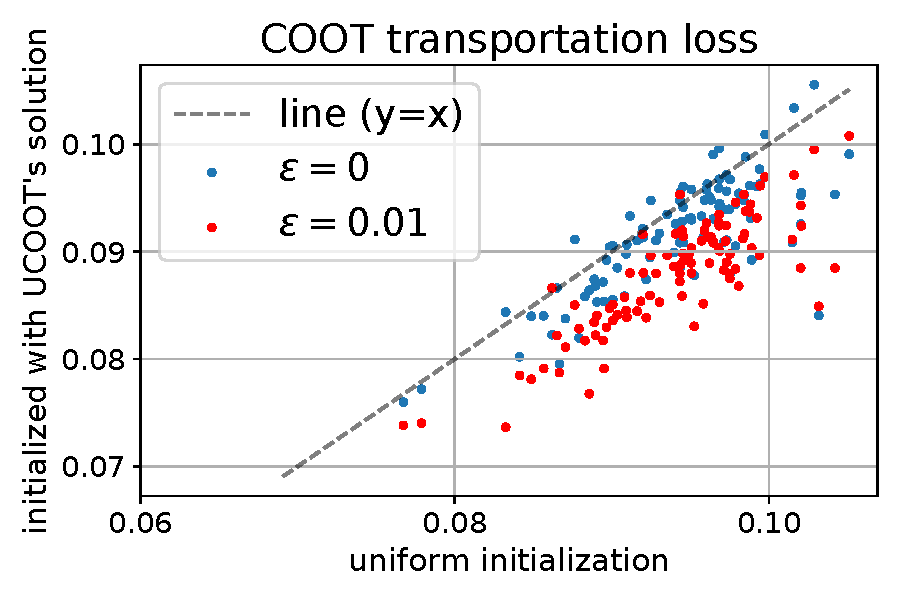
\includegraphics[width=\linewidth]{./Chapitre3/fig/init.pdf}
  \vspace*{-10mm}
  \caption{Scatter plot of the COOT transportation cost with naive initialization (y-axis)
  vs initialization with UCOOT.
  \label{fig:init}}
\end{wrapfigure}
Interestingly, we find that COOT can achieve better minima when initialized with the UCOOT solutions.
\Cref{fig:init} illustrates how UCOOT can lead to better alignments by finding
better local minima of the COOT transportation cost. For 100 random Gaussian datasets
$A, B$ with uniformly sampled shapes $n_1, n_2, d_1, d_2$, we visualize the COOT loss
with uniform initialization (y-axis) versus the COOT loss when initializing the COOT BCD
with UCOOT's solution. For both $\varepsilon = 0$ and $\varepsilon > 0$,
the latter leads to lower COOT costs than the former, on average.

As COOT is a non-convex problem, the choice of initialization plays an important role.
Intuitively, by choosing $\lambda_1$ and $\lambda_2$ sufficiently large,
one can use UCOOT to approach COOT. For this reason, the solution of UCOOT can be more informative
than the usual uniform initialization, and one can expect to reach better local optimal of COOT.

%%%%%%%%%%%%%%%%%%%%%%%%%%%%%%%%%%
\subsection{Experimental details} \label{sec_app:exp}

\subsubsection{More details on barycentric mapping}  \label{bary_mapping}

The barycentric mapping \citep{Ferradans14,Courty16} is a method to transform the source data
to the target domain. Given the source data $X_s \in \bbR^{n_s \times d_s}$ and
target data $X_t \in \bbR^{n_t \times d_t}$, once the optimal transportation plan
$P \in \bbR^{n_s \times n_t}$ is learned, the transformation of the source to the target domain,
can be expressed as: for $i = 1, ..., n_s$,
\begin{equation} \label{bary_optim}
    \widehat{x}_i^{(s)} \in \argmin_{x \in \bbR^{d_t}}
    \sum_{j = 1}^{n_t} P_{ij} \; c(x, x_j^{(t)}),
\end{equation}
where the example $x^{(t)}_j \in \bbR^{d_t}$ corresponds to the $j$-th row of $X_t$ and
the cost $c: \bbR^{d_t} \times R^{d_t} \to \bbR$ measures the discrepancy between
two examples in $\bbR^{d_t}$. Typically, $c$ is the squared Euclidean distance,
so Problem \eqref{bary_optim} admits a closed form solution, which is a weighted average of
examples in the target domain:
\begin{equation}
    \widehat{x}_i^{(s)} = \sum_{j = 1}^{n_t} \frac{P_{ij}}{p_i} x_j^{(t)},
\end{equation}
where $p_i = \sum_{j} P_{ij}$, or in matrix notation:
\begin{equation} \label{transOT:1}
    \widehat{X}_s= \diag(\frac{1}{P 1_{n_t}}) P X_t \in \bbR^{n_s \times d_t},
\end{equation}
where the division is element-wise.

\subsubsection{Heterogenous Domain Adaptation (HDA)}
\paragraph{More details on label propagation}

Once the sample coupling $P$ is learned, the label propagation works as follows:
suppose the labels contain $K$ different classes,
we apply the one-hot encoding to the source label $y^{(s)}$ to obtain
$D^{(s)} \in \bbR^{K \times n_s}$ where $D^{(s)}_{ki} = 1_{\{y^{(s)}_i = k\}}$.
The label proportions on the target data are
estimated by: $L = D^{(s)} P \in \bbR^{K \times n_t}$. Then the prediction can be generated
by choosing the label with the highest proportion, \ie, $\widehat{y}^{(t)}_j = \argmax_k L_{kj}$.

\paragraph{Paramater validation}

We tune the hyperparameters of each method via grid search.
\begin{itemize}
  \item[$\bullet$] For COOT, we choose the regularisation on the feature and sample couplings
  $\varepsilon_f, \varepsilon_s \in \{0, 0.01, 0.1, 0.5\}$.
  \item[$\bullet$] For GW, we choose the regularisation parameter
  $\varepsilon \in \{0, 0.001, 0.005, 0.01, 0.05, 0.1, 0.5\}$.
  \item[$\bullet$] For UGW and UCOOT, we choose $\lambda_1, \lambda_2 \in \{1, 5, 20, 50\}$ and
  $\varepsilon \in \{0.01, 0.05, 0.1, 0.5\}$.
  Furthermore, for UGW and GW, before calculating the Euclidean distance matrix for each domain,
  the matrix of domain data is normalised by max scaling, so that its coordinates are bounded in
  $[-1,1]$. This pre-processing step improves the performance of the for UGW and GW.
\end{itemize}
For each method, for each combination of tuple of hyperparameters, first, we choose a pair
amongst $9$ pairs, then repeat $10$ times the training procedure, in which the optimal plan
is estimated, then used to calculate the accuracy. We choose the tuple of hyperparameters
corresponding to the highest average accuracy. This optimal tuple is then applied to
all other $8$ tasks, where in each task, the training procedure is repeated $10$ times and
we report the average accuracy.

\paragraph{When there is no regularization} In the above hyperparameter tuning process,
we only considered $\varepsilon > 0$ for UCOOT and UGW, so that the scaling algorithm
\citep{Chizat18b} is applicable. We note that,
the MM solver can allow us to handle the case $\varepsilon = 0$
(\ie, we can estimate directly UCOOT, rather than via its entropic approximation).
In this case, we also tune $\lambda_1, \lambda_2 \in \{ 1, 50, 20, 50\}$ and
follow exactly the same tuning and testing procedure as in the case $\varepsilon > 0$.
We report our finding in \Cref{tab:hda2}. We observe that, in many tasks,
the performance remains competitive while enjoying lower variance.
\newline
\begin{table}[h]
	\begin{center}
		\begin{small}
			\begin{sc}
				\begin{tabular}{c c c c c}
					\toprule
					& \multicolumn{2}{c}{CaffeNet $\to$ GoogleNet} \\
					\midrule
					Domains & COOT & UCOOT ($\varepsilon > 0$) & UCOOT ($\varepsilon = 0$) \\
					\midrule

					C $\to$ C & 36.40 ($\pm$ 12.94) & \textbf{44.05 ($\pm$ 19.33)} & 38.60 ($\pm$ 9.16) \\
					\hline
					C $\to$ A & 28.30 ($\pm$ 11.78) & \textbf{31.90 ($\pm$ 7.43)} & 29.45 ($\pm$ 9.94) \\
					\hline
					C $\to$ W & 19.55 ($\pm$ 14.51) & 28.55 ($\pm$ 6.60) & \textbf{40.85 ($\pm$ 12.53)} \\
					\hline

					A $\to$ C & \textbf{41.80 ($\pm$ 14.81)} & 39.15 ($\pm$ 17.98) & 18.00 ($\pm$ 9.22) \\
					\hline
					A $\to$ A & \textbf{57.90 ($\pm$ 16.84)} & 42.45 ($\pm$ 15.47) & 40.40 ($\pm$ 8.40) \\
					\hline
					A $\to$ W & 42.10 ($\pm$ 7.80) & 48.55 ($\pm$ 13.06) & \textbf{49.15 ($\pm$ 6.64)} \\
					\hline

					W $\to$ C & 8.60 ($\pm$ 6.56) & \textbf{69.80 ($\pm$ 14.91)} & 19.70 ($\pm$ 5.79) \\
					\hline
					W $\to$ A & 16.65 ($\pm$ 10.01) & \textbf{30.55 ($\pm$ 10.09)} & 25.90 ($\pm$ 5.48) \\
					\hline
					W $\to$ W & \textbf{75.30 ($\pm$ 3.26)} & 51.50 ($\pm$ 20.51) & 49.55 ($\pm$ 6.02) \\
					\bottomrule
					Average & 36.29 ($\pm$ 10.95) & \textbf{42.94 ($\pm$ 13.93)} & 34.62 ($\pm$ 11.17) \\
					\bottomrule

				\end{tabular}
			\end{sc}
		\end{small}
	\end{center}
	\caption{Unsupervised HDA from CaffeNet to GoogleNet for $\varepsilon > 0$ and $\varepsilon = 0$.
  UCOOT ($\varepsilon > 0$) corresponds to the model where $\varepsilon, \lambda_1$ and $\lambda_2$
  are tuned, with $\varepsilon > 0$, and UCOOT ($\varepsilon = 0$) means that $\varepsilon = 0$
  and only $\lambda_1, \lambda_2$ are tuned. }
	\label{tab:hda2}
\end{table}

\paragraph{Sensitivity analysis}
We report the sensitivity of UCOOT's performance to the hyper-parameters $\varepsilon, \lambda_1$
and $\lambda_2$ for two tasks C$\to$W and A$\to$A in
\Cref{tab:sensitiv_eps,tab:sensitiv_lambda1,tab:sensitiv_lambda_2}. In general,
the performance depends significantly on the choice of hyperparameters.
In \Cref{tab:sensitiv_eps}, given fixed values of $\lambda_1$ and $\lambda_2$,
UCOOT performs badly for either too small or large values of $\varepsilon$,
indicating that regularization is necessary but should not be too strong.
From \Cref{tab:sensitiv_lambda1}, we see that large value of $\lambda_1$ degrades
the performance, meaning that the marginal constraints on the source distributions should not
be too tight. Meanwhile, it seems that large $\lambda_2$ is preferable,
so the marginal distributions on the target spaces should not be too relaxed.

\hfill
\begin{table}[H]
	\begin{center}
		\begin{footnotesize}
			\begin{sc}
				\begin{tabular}{c c c c c c c}
					\toprule
					& \multicolumn{5}{c}{CaffeNet $\to$ GoogleNet} \\
					\midrule
					Domains & $\varepsilon= 0.03$ & 0.05 & 0.1 & 0.2 & 0.4 \\
					\midrule
					C $\to$ W & 27.65 ($\pm$ 11.34) & 37.20 ($\pm$ 9.35) & 34.75 ($\pm$ 13.04) & 17.00 ($\pm$ 5.92) & 11.25 ($\pm$ 1.66) \\
					\hline
					A $\to$ A & 21.95 ($\pm$ 9.46) & 35.30 ($\pm$ 15.11) & 41.15 ($\pm$ 19.16) & 58.45 ($\pm$ 15.54) & 8.90 ($\pm$ 1.34) \\
					\hline
				\end{tabular}
			\end{sc}
		\end{footnotesize}
	\end{center}
	\caption{Sensitivity of UCOOT to $\varepsilon$ in tasks C$\to$W and A$\to$A.
  We fix $\lambda_2 = 50$ and $\lambda_1 = 1$ and show the accuracy for various value of
  $\varepsilon$.} \label{tab:sensitiv_eps}
\end{table}
%%%%%%%%%%%%%%%%%

\hfill
\begin{table}[H]
	\begin{center}
		\begin{footnotesize}
			\begin{sc}
				\begin{tabular}{c c c c c c c}
					\toprule
					& \multicolumn{5}{c}{CaffeNet $\to$ GoogleNet} \\
					\midrule
					Domains & $\lambda_1= 20$ & 40 & 50 & 60 & 80 \\
					\midrule
					C $\to$ W & 35.80 ($\pm$ 9.33) & 37.35 ($\pm$ 13.82) & 27.45 ($\pm$ 8.33) & 32.45 ($\pm$ 11.62) & 30.15 ($\pm$ 12.89) \\
					\hline
					A $\to$ A & 55.20 ($\pm$ 18.44) & 44.15 ($\pm$ 21.54) & 24.30 ($\pm$ 15.58) & 36.10 ($\pm$ 23.97) & 24.80 ($\pm$ 15.08) \\
					\hline
				\end{tabular}
			\end{sc}
		\end{footnotesize}
	\end{center}
	\caption{Sensitivity of UCOOT to $\lambda_1$ in tasks C$\to$W and A$\to$A.
  We fix $\lambda_2 = 1$ and $\varepsilon = 0.1$ and show the accuracy for various value of
  $\lambda_1$.} \label{tab:sensitiv_lambda1}
\end{table}
%%%%%%%%%%%%%%

\hfill
\begin{table}[H]
	\begin{center}
		\begin{footnotesize}
			\begin{sc}
				\begin{tabular}{c c c c c c c}
					\toprule
					& \multicolumn{5}{c}{CaffeNet $\to$ GoogleNet} \\
					\midrule
					Domains & $\lambda_2= 0.3$ & 0.5 & 1 & 2 & 4 \\
					\midrule
					C $\to$ W & 34.20 ($\pm$ 9.83) & 34.45 ($\pm$ 10.80) & 34.75 ($\pm$ 13.04) & 29.70 ($\pm$ 10.55) & 32.30 ($\pm$ 18.81) \\
					\hline
					A $\to$ A & 20.75 ($\pm$ 10.11) & 29.00 ($\pm$ 15.79) & 41.15 ($\pm$ 19.16) & 32.65 ($\pm$ 8.80) & 49.95 ($\pm$ 15.75) \\
					\hline
				\end{tabular}
			\end{sc}
		\end{footnotesize}
	\end{center}
	\caption{Sensitivity of UCOOT to $\lambda_2$ in tasks C$\to$W and A$\to$A.
  We fix $\lambda_1 = 50$ and $\varepsilon = 0.1$ and show the accuracy for various value of
  $\lambda_2$.} \label{tab:sensitiv_lambda_2}
\end{table}

\paragraph{Additional results}
We also perform the adaptation from GoogleNet to CaffeNet. The results can be found in
\Cref{tab:table3}. We draw the same conclusions as in the adaptation from CaffeNet to GoogleNet.

\hfill
\begin{table}[H]
  \begin{center}
    \begin{small}
      \begin{sc}
        \begin{tabular}{c c c c c}
          \toprule
          & \multicolumn{3}{c}{GoogleNet $\to$ CaffeNet} \\
          \midrule
          Domains & GW & UGW & COOT & UCOOT \\
          \midrule

          C $\to$ C & 19.45 ($\pm$ 10.88) & 17.50 ($\pm$ 4.88) & 46.20 ($\pm$ 14.94) & \textbf{46.50 ($\pm$ 5.81)} \\
          \hline
          C $\to$ A & 9.35 ($\pm$ 7.73) & 10.50 ($\pm$ 7.06) & 33.25 ($\pm$ 17.56) & \textbf{34.45 ($\pm$ 4.89)} \\
          \hline
          C $\to$ W & 19.15 ($\pm$ 10.59) & 11.95 ($\pm$ 7.49) & 14.95 ($\pm$ 12.44) & \textbf{33.60 ($\pm$ 10.07)} \\
          \hline

          A $\to$ C & 7.90 ($\pm$ 4.92) & 11.70 ($\pm$ 5.57) & 28.80 ($\pm$ 12.02) & \textbf{40.55 ($\pm$ 6.50)} \\
          \hline
          A $\to$ A & 19.75 ($\pm$ 9.51) & 18.40 ($\pm$ 11.71) & \textbf{59.30 ($\pm$ 20.77)} & 58.95 ($\pm$ 10.37) \\
          \hline
          A $\to$ W & 14.55 ($\pm$ 14.62) & 10.05 ($\pm$ 4.70) & 9.75 ($\pm$ 7.75) & \textbf{65.20 ($\pm$ 9.80)} \\
          \hline

          W $\to$ C & 14.05 ($\pm$ 5.97) & 21.95 ($\pm$ 4.33) & 13.70 ($\pm$ 7.01) & \textbf{33.45 ($\pm$ 6.67)} \\
          \hline
          W $\to$ A & 22.85 ($\pm$ 11.87) & 20.90 ($\pm$ 5.98) & \textbf{47.70 ($\pm$ 5.53)} & 44.45 ($\pm$ 6.02) \\
          \hline
          W $\to$ W & 24.10 ($\pm$ 15.78) & 27.95 ($\pm$ 8.34) & \textbf{72.55 ($\pm$ 4.82)} & 68.80 ($\pm$ 10.24) \\
          \bottomrule
          Average & 16.79 ($\pm$ 10.21) & 16.77 ($\pm$ 6.67) & 36.24 ($\pm$ 11.43) & \textbf{47.33 ($\pm$ 7.82)} \\
          \bottomrule
        \end{tabular}
      \end{sc}
      \end{small}
  \end{center}
  \caption{Unsupervised HDA from GoogleNet to CaffeNet.}
  \label{tab:table3}
\end{table}

%%%%%%%%%%%%%%%%%%%%%%%%%%%%%%
\subsubsection{Multi-omic dataset alignment}\label{multiOmics_exp_SI}

\paragraph{Data Preprocessing} \label{CITEseq_exp_appendix}
For the single-cell multi-omics experiments, we use the ``PBMC'' dataset from Stoeckius
\textit{et al} \citep{CITEseq}, accessed on Gene Expression Omnibus (GEO) with the
accession code: \href{https://www.ncbi.nlm.nih.gov/geo/query/acc.cgi?acc=GSE100866}{GSE100866}.
This dataset contains a mix of 7,985 mouse and human peripheral blood mononuclear cells (PBMC)
and profiles ten antibodies, 17,014 human genes, and 12,915 mouse genes. To pick the human cells,
we follow the description in \citep{CITEseq}, and select the cells that have at least 500,
and more than 90\% of all unique molecular identifiers (UMIs) mapped to the human genes
(rather than the mouse genes). From the resulting $\sim 4500$ cells, we pick the first 1000
to use in our experiments. We use the CLR-normalized antibody count data provided in GEO
and apply log normalization to the gene expression data using Seurat package in R to
remove biases in sequencing across cells \citep{Seurat}. Prior to alignment,
we follow the existing single-cell alignment methods \citep{Demetci22, Demetci22-2,Liu2019,singh20},
and also apply L2 normalization to both modalities. The top 50 most variable genes
(\Cref{fig:multiomics}(c)) are selected using the \texttt{FindVariableFeatures()}
function from \citep{Seurat}.

\paragraph{Hyperparameter tuning} Hyperparameters were tuned using grid search.
For both COOT and UCOOT, we considered the following range for the entropic regularization
coefficients $\varepsilon_f, \varepsilon_s \in \{1e-5, 5e-5, 1e-5, 5e-4, ... ,0.1, 0.5\}$.
For the mass relaxation coefficients $\lambda_1, \lambda_2 $ in UCOOT, the following range
was considered $\lambda_1, \lambda_2 \in \{1e-3, 5e-3, 0.01, 0.05, 0.1, 0.5, 1, 5, 10, 50 ,100\}$.
Each combination of hyperparameters were run on three randomly chosen subsets of the dataset
that included 30\% of the samples and the hyperparameter combinations that on average yielded
the highest feature matches and lowest FOSCTTM were picked for the experiments on the full dataset.
Below, we list the hyperparameter combinations used for the final alignment results
reported in this paper:
\begin{itemize}
    \item[$\bullet$] \textbf{Balanced scenario of aligning matching features
    (\Cref{fig:multiomics}(a)):} \\ $\lambda_1=1, \lambda_2=0.1, \varepsilon_1=1e-4, \varepsilon_2=1e-4$
    \item[$\bullet$] \textbf{Unbalanced scenario of aligning a subset of the matching features
    (\Cref{fig:multiomics}(b)):} \\ $\lambda_1=1, \lambda_2=1e-2, \varepsilon_1=1e-4, \varepsilon_2=1e-4$
    \item[$\bullet$] \textbf{Unbalanced scenario of aligning antibodies with the top 50 most variable genes
    (\Cref{fig:multiomics}(c)):}  $\lambda_1=10, \lambda_2=5e-5, \varepsilon_1=1e-4, \varepsilon_2=0.5$
    \item[$\bullet$] \textbf{Balanced scenario of aligning the same number of cells
    (\Cref{fig:multiomicsSamples}(a)):} \\ $\lambda_1=1, \lambda_2=0.1, \varepsilon_1=1e-4, \varepsilon_2=1e-4$
    \item[$\bullet$] \textbf{Unbalanced scenario 1 of aligning different number of cells
    (\Cref{fig:multiomicsSamples}(b)):} \\ $\lambda_1=0.01, \lambda_2=0.1, \varepsilon_1=5e-3, \varepsilon_2=1e-4$
    \item[$\bullet$] \textbf{Unbalanced scenario 2 of aligning different number of cells
    (\Cref{fig:multiomicsSamples}(c)):} \\ $\lambda_1=0.01, \lambda_2=0.1, \varepsilon_1=5e-3, \varepsilon_2=1e-4$
\end{itemize}

\paragraph{Further investigation of the feature alignments}
In the unbalanced experiment, where we align the most variable genes and the antibodies,
we expect a well-performing alignment method to correctly match antibodies with the genes
that express them. This would be the strongest biological connection between a protein
(\ie, an antibody, in this case) and a gene. However, other biological connections can also exist,
such as between an antibody and a gene that regulates the expression of that antibody,
a gene that codes for a protein the antibody physically interacts with, or a gene that codes
for a protein that is active in the same biological pahtway as the antibody of interest.
To investigate whether there are such matches recovered outside of the ten genes we label
as ``matching genes'', we refer to two gene regulatory network databases that contain data
on human PBMCs, GRNdb \citep{GRNdb} and GRAND \citep{GRAND} (for the first kind of relationship),
two protein--protein interaction databases, BioGRID \citep{BIOGRID}, and STRING \citep{STRING}
(for the second kind of relationship), and KEGG \citep{KEGG}, a database of biological pathways
(for the last kind of relationship).

Of the 46 correspondences yielded by COOT, and 16 by UCOOT, outside of the
`correspondences with `matching genes'', only a few show up on these databases:
\begin{itemize}
    \item[$\bullet$] \textbf{CD19 antibody correspondences:} Both BIOGRID \citep{BIOGRID} and
    STRING \citep{STRING} databases return a physical interaction with CD79A protein
    (encoded by the \textit{CD79A} gene), which is experimentally validated by
    affinity capture-Western \citep{Carter97}. The correspondence with \textit{CD79A} is yielded
    by both UCOOT and COOT. Additionally, according to KEGG \citep{KEGG},
    CD19 participates in the B-cell receptor (BCR) signaling pathway along with IGH,
    which is formed by multiple segments joining together, including IGHD and
    IGHM \footnote{\url{https://www.genecards.org/cgi-bin/carddisp.pl?gene=IGHD},
    and \url{https://www.genecards.org/cgi-bin/carddisp.pl?gene=IGH&keywords=IGH}}.
    COOT yields correspondences with the genes that code for these.

    \item[$\bullet$] \textbf{CD57 antibody correspondences:} There is an experimentally validated
    physical interaction with ITM2C (encoded by the \textit{ITM2C} gene), which shows up on BIOGRID.
    This interaction has been validated using proximity labeling mass spectrometry \citep{Go2021}.
    \textit{ITM2C} is among the correspondences yielded by COOT.

    \item[$\bullet$] \textbf{CD2 antibody correspondences:} According to the BIOGRID database,
    a physical interaction between CD2 and PTPRC has been proposed via an \textit{in vitro}
    study \textit{et al} \citep{Schraven90}. \textit{PTPRC} shows up among the correspondences
    yielded by both UCOOT and COOT for the CD2 antibody.

    \item[$\bullet$] \textbf{CD4 antibody correspondences:} According to BIOGRID, CD4 has been shown
    to physically interact with TUBB using affinity capture mass spectrometry by
    Bernhard \textit{et al} \citep{Bernhard2004}. TUBB is a component of the tubulin protein,
    which made out of $\beta-$tubulin (TUBB) and $\alpha-$tubulin (TUBA).
    UCOOT yields a correspondence between CD4 and TUBA1B (gene that codes for a component
    of the $\alpha-$tubulin)
    \footnote{\url{https://www.nature.com/scitable/content/microtubules-the-basics-14673338/}}.
\end{itemize}
Outside of these, no other correspondences returned biological relevance based on our database and
literature search, which leads us to conclude COOT yields more redundant correspondences that UCOOT.

\paragraph{Sample alignment experiments} Below in \Cref{fig:multiomicsSamples},
we visualize the aligned samples (first two principal components of the two domains
together upon barycentric projection) and report the alignment performance as measured
by the ``average fraction of samples closer than true match (FOSCTTM)'' and
``label transfer accuracy'' metrics. We borrow these metrics from previously published
single-cell multi-omic data alignment methods \citep{Liu2019,cao2020unsupervised,Demetci22,Pamona,Demetci22-2}.
For label transfer accuracy, we follow the previously published methods
\citep{cao2020unsupervised, Pamona, Demetci22, Demetci22-2} and train a $k-$NN classifier
(for $k=5$) on the cell-type labels of the measurement domain with the full set of cells,
and apply it to predict the cell-type labels of the downsampled domain.
We report the prediction accuracy. For the balanced scenario, we train the classifier
on the antibody domain to predict the labels in the gene expression domain upon transportation.
For the average FOSCTTM metric used in unbalanced scenarios, we use the cells that
remain to have a correspondence after subsampling to calculate the FOSCTTM scores.
We note that lower average FOSCTTM and higher label transfer accuracy results indicate
better alignments.

\begin{figure}[h]
    \centering
    \includegraphics[width=\linewidth]{./Chapitre3/fig/citeseq-samples.pdf}
    % \includegraphics[width=.8\linewidth,trim={0 0 15cm 0},clip]{fig/citeseq-samples.pdf}
    \caption{Visualization of the sample alignments with UCOOT and COOT after
    barycentric projection (First two principal components). The top row visualizes results
    with samples colored based on measurement modality (black points show the
    gene expression domain samples, and red points show the antibody domain samples).
    The bottom row visualizes alignments with samples colored based on cell-type labels.
    \textbf{(a)} presents sample alignments in the balanced scenario, where we align
    the same number of cells (1000) in each measurement modality with the matching features
    (same scenario as Fig 6 (a), but presenting sample alignments).
    \textbf{(b)} In this unbalanced scenario, we randomly downsample
    the cells in antibody domain by 25\%.
    \textbf{(c)} In this second unbalanced scenario, we randomly downsample the cells
    in the gene expression domain by 25\% and align with the full set of samples
    in the antibody domain. For all alignments, we quantify alignment quality using
    average FOSCTTM (``Ave. FOSCTTM'') and label transfer accuracy (``Label Tr. Acc.''),
    and report them under the plots. We calculate both metrics prior to applying
    dimensionality reduction with principal component analysis (PCA).
    PCA is only applied for visualization purposes. Note that the overall increase in
    label transfer accuracy between \textbf{a-c} is likely due to the removal of
    groups of heterogenous cell types during downsampling.
    \label{fig:multiomicsSamples}
  }
\end{figure}